<<<<<<< HEAD
% !TeX encoding = UTF-8
% !TeX program = pdflatex
% !BIB program = bibtex

% Use Packages
\usepackage{graphicx}

%%% Um einen Artikel auf deutsch zu schreiben, genügt es die Klasse ohne
%%% Parameter zu laden.
=======
>>>>>>> 4e4bcdda93ef5b884d3aa359162611458d088d35
\documentclass[]{lni}

\usepackage{graphicx}
\graphicspath{{./Bilder/}}

\begin{document}

    \title[SUBSCALE]{SUBSCALE Algorithmus}
%%%\subtitle{Untertitel / Subtitle} % if needed
    \author[William Mendat \and Max Ernst \and Steven Schall \and Matthias Reichenbach]
    {William Mendat\footnote{Hochschule Offenburg, Offenburg,
        Deutschland \email{wmendat@stud-hs.offenburg.de}} \and
    Max Ernst\footnote{Hochschule Offenburg, Offenburg,
        Deutschland \email{wmendat@stud-hs.offenburg.de}} \and
    Steven Schall\footnote{Hochschule Offenburg, Offenburg,
        Deutschland \email{sschall@stud-hs.offenburg.de}} \and
    Matthias Reichenbach\footnote{Hochschule Offenburg, Offenburg,
        Deutschland \email{mreichen@stud-hs.offenburg.de}}}
    \startpage{1} % Beginn der Seitenzählung für diesen Beitrag / Start page
<<<<<<< HEAD
    \editor{Team Subscale} % Names of Editors
    \booktitle{Subscale Algorythmus} % Name of book title
=======
    \editor{Team SUBSCALE} % Names of Editors
    \booktitle{SUBSCALE Algorithmus} % Name of book title
>>>>>>> 4e4bcdda93ef5b884d3aa359162611458d088d35
    \yearofpublication{2022}
    \maketitle

    \begin{abstract}
    Das könnte das abstract sein
\end{abstract}
\begin{keywords}
    C++ \and Subscale \and Cluster %Keyword1 \and Keyword2
\end{keywords}
    \section{Einleitung}
Der Subscale-Algorithmus ist eine effiziente, parallelisier- und folglich auch verteilbare Methode zur Ermittlung von
Clustern in hochdimensionalen Räumen. Ziel des Projektes ist eine Implementierung des Algorithmus, welche sich auf
mehreren geclusterten Maschinen verteilen lässt, um die Clusterermittlung mit einer hohen GPU-Rechenkapazität zu
beschleunigen.

    \section{Analyse des Algorithmus}
Clustering-Algorithmen suchen in vieldimensionalen Räumen nach Gruppen von Einträgen mit ähnlichen Eigenschaften. Hierbei werden die Eigenschaften eines Datensatzes, im Folgenden \glqq Features\grqq genannt, als numerischer Vektor repräsentiert und mit denen anderer Datensätze mit einem geeigneten Distanzmaß verglichen. Die Hyperparameter $\tau$ und $\epsilon$ bestimmen, wann es sich bei ähnlichen Datensätzen um ein Cluster handelt. $\epsilon$ ist die Maximaldistanz, welche zwei Datensätze haben dürfen, um ähnlich zu sein. $\tau$ bestimmt die Minimalgröße eines Clusters. Ein Cluster besteht folglich aus mindestens $\tau$ Datensätzen, welche einen Maximalabstand von $\epsilon$ zueinander haben.\\
Der Subscale-Algorithmus unterscheidet sich von gängigen Clustering-Algorithmen dadurch, dass er Teilräume der Datensätze miteinander vergleicht. Diese speicherintensive Methode gliedert sich in sieben Schritte, welche sich jeweils parallelisieren und verteilen 
lassen.

\subsection{Aufbereitung der Daten}
Initial wird jedes Datum mit einer hohen zufälligen Ganzzahl markiert. Dieser Schlüssel dient in einem späteren Schritt zur Kollisionsdetektion mittels Hashtabelle. Die Summe mehrerer Schlüssel bildet mit einer hohen Wahrscheinlichkeit einen eindeutigen Wert, 
welcher dann als Vergleichselement genutzt werden kann.

\subsection{Core-Set Erzeugung}
Zunächst wird jede Dimension isoliert betrachtet. Das bedeutet, das ein bestimmtes Feature eines jeden Datensatzes mit dem gleichen Feature der anderen Datensätze mit einem geeigneten Distanzmaß verglichen wird. Sind sich mindestens $\tau$ Datensätze $\epsilon$ nahe oder näher, bilden diese Datensätze ein Core-Set. Die Core-Sets sind eindimensionale Cluster und werden für jede Dimension ermittelt.

\subsection{Kombination zu Dense Units}
Die Core-Sets werden weiter prozessiert. Jegliche mögliche Kombination aus Punkten eines Core-Sets mit der Größe $\tau$ bilden eine Dense Unit. Dense Units werden für jedes Core-Set in jeder Dimension kombiniert.

\subsection{Dense Unit Kollision}
In diesem Schritt werden die Dense Units einer Dimension mit deren anderer Dimensionen verglichen. Der Vergleich geschieht mittels des initial zugewiesenen Schlüssels. Die Summe der Schlüssel aller Features einer Dense Unit bildet die Signatur der Dense Unit. Diese Signatur ist aufgrund der hohen Schlüsselwerte mit hoher Wahrscheinlichkeit eindeutig. Durch den Vergleich von Dense Unit Signaturen kann somit effizient ermittelt werden, ob die gleiche Dense Unit in unterschiedlichen Dimensionen existiert. Dense Unit Paare werden mit den Dimensionen, in welchen sie vorkommen, gelabelt.

\subsection{Subspacing}
Punkte aus Dense Units mit identischen Dimensionslabels werden im Subspacing-Schritt aggregiert. Das so ermittelte Set an Punkte ist ein möglicher Clusterkandidat.

\subsection{Cluster Detection mit DBSCAN}
Die Cluster der Daten werden im finalen Schritt mit dem Clustering-Algorithmus DBSCAN ermittelt. DBSCAN erhält lediglich den durch die vorherigen Schritte bereinigten Datensatz und kann aus diesem in endlicher Zeit Cluster ermitteln.
    \section{Berechnung der Dense Units}
\label{sec:chap3}

Clusters von benachbarten Punkten müssen zu einem minPoint Großen subsets kombiniert werden. Diese subsets werden Dense Units genannt.
Dense Units werden in verschiedene Funktionen mit unterschiedlichen Zwecken berechnet. Das Hauptziel dieser Berechnung, ist die Bestimmung einer Teilmenge aus allen möglichen Kombinationen in einem subset. Dabei dürfen keine Wiederholungen der Dense Units auftreten. Die Kombinationen aus einem subset können mittels dem Binominialkoeffizient berechnen, $ \binom{n}{k} $ dabei ist n die Anzahl der Elemente in dem subset und k die minimale Anzahl an punkten in einem subset (e.g. minPoints). Daraus entstehen k-Elemente großes subsets von einem n-Elemente set ohne Wiederholungen der Kombinationen.
Wenn zum Beispiel ein Core Set aus folgenden Punkten besteht: [1, 5, 7, 9, 22] und die minimale Anzahl an punkten in einem Subset Drei ist, sind die ersten Drei Dense Units folgende: [1, 5, 7] und [1, 5, 9] und [1, 5, 22]. Die Formel zur Berechnung der Dense Units kann also folgendermaßen betrachtet werden: 
$ \binom{|CS|}{minPoints}$ \cite{7022654} Abbildung \ref{dense-calculation} zeigt ein weiteres Beispiel für n-Punkte in einem Core Set mit minPoints von 4.

\begin{figure}
	\centering
	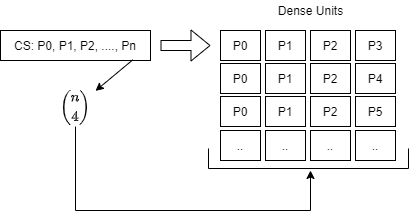
\includegraphics[width=0.5\textwidth]{DenseUnitBerechnung.png}
	\caption{Berechnung der Dense Units}
	\label{dense-calculation}
\end{figure}
    
\section{Codebasis Umstrukturierung}

Wir haben uns dann als Team dazu entschlossen, dass die eigene Implementierung gescheitert war und etwas anderes versucht werden musste.
Die Idee war es, die vorhandene Implementierung zu nutzen, aber da der Code sehr schwer zu verstehen war und auch die Zeit so langsam ein 
Problem wurde, nur noch die Slices auf einem Cluster zu parallelisieren. Das Vorgehen dabei war es, den vorhandenen Code nicht wirklich zu 
verändern sondern, nur die vorhandenen Funktionen wieder zu verwenden. 
\newline 
\newline 
Der originale Code hatte eine Klasse \emph{LocalSubspaceTable}, die für das Darstellen der \emph{Subspace}-Tabelle zuständig war.
Diese Klasse wurde sowohl für die \emph{Slices} als auch für die gesamten \emph{Subspaces} verwendet. Meine Idee war es dann,
den anderen im Team eine Funktion names \emph{calculateRemote} bereitzustellen, die als Parameter die \emph{Labels}, den \emph{minBound} des Slices und den 
\emph{maxBound} des Slices bekommt und den berechneten Slice als Form der \emph{LocalSubspaceTable}-Klasse zurückgibt. 
\newline
\newline
Im Folgenden wird zunächst der Aufbau des originalen Code erläutert, um anschließend die Umsetzung der \emph{calculateRemote}-Methode
von unten nach oben darzustellen. 

\subsection{Aufbau des originalem Code}
Der Code bestand im wesentlichen aus einer abstrakten Klasse \emph{ISubscale} und zwei konkreten Implementierungen
\emph{Subscale} (\emph{Cuda}-Implementation) und \emph{SubscaleSec} (normale Implementation) wie im folgenden gezeigt:
\newpage
\begin{figure}[h]
    \centering
    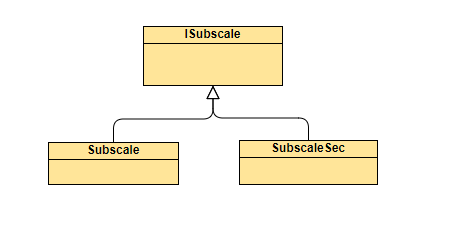
\includegraphics[width=\textwidth]{Subscale.png}
    \caption{Subscale}
    \label{img:subscale}
\end{figure}

\emph{ISubscale} selber hatte eine Funktion \emph{calculateClusterCandidates} die Vorbereitungen getroffen hat und die 
konkrete Implementierung sollte die Funktion \emph{calculateAllSlices} überschreiben, die den Zweck hatte, alle \emph{Slices}
zu erstellen und auf die Festplatte zu schreiben. Außerdem verfügte \emph{ISubscale} noch über eine Funktion \emph{combineAllSlices}
die die einzelnen Slices von der Festplatte geholt hat, die Slice verengert hat und dann zu der endgültigen Subspace Tabelle 
hinzugefügt hat.   

\subsection{calculateSlice}
Angefangen am untersten Ende brauchten die beiden konkreten Implementationen eine neue Funktion, die alle nötigen Informationen 
bekommt, um einen Slice zu erstellen und als Rückgabe dann den Slice zurückgibt. Da sich die konkreten Implementationen nur in der 
Erzeugung der konkreten Klassen unterscheidet, wird in dieser Section der generelle Code gezeigt und in den folgenden Abschnitten 
nur die wesentlichen Unterschiede.  

\lstinputlisting[language=C++,caption={calculateSlice},
    label=lst:calculateSlice]{src/calculateSlice.cpp}

Wie in Listing \ref{lst:calculateSlice} zu sehen ist, werden die Berechungsklassen initialisiert und anschließend werden die 
\emph{DenseUnits} erzeugt, um diese dann in eine Subspace Tabelle hinzuzufügen. Sollte der \emph{Slice} nicht leer sein, dann 
werden die Einträge noch nach den Subspaces zusammengefügt. Als letztes wird noch der Speicher von der Grafikkarte zum Host kopiert 
(ist bei der sequentiellen Abarbeitung nicht nötig). 

\subsection{calculateSlice Sequentiell}
In dieser Sektion werden noch die spezifischen Erzeugungen der Berechungsklassen für die Sequentielle Abarbeitung gezeigt.

\lstinputlisting[language=C++,caption={calculateSlice Sequentiell},
    label=lst:calculateSliceSeq]{src/calculateSliceSeq.cpp}

\subsection{calculateSlice Sequentiell}
In dieser Sektion werden noch die spezifischen Erzeugungen der Berechungsklassen für die \emph{Cuda} Abarbeitung gezeigt.

\lstinputlisting[language=C++,caption={calculateSlice Cuda},
    label=lst:calculateSliceCuda]{src/calculateSliceCuda.cpp}

\subsection{calculateClusterCandidatesRemote}
Die nächst obere Stufe war die \emph{calculateClusterCandidatesRemote}-Methode, die alle notwendigen 
Informationen für die \emph{calculateSlice} vorbereitet. Diese sieht wie folgt aus:

\lstinputlisting[language=C++,caption={calculateClusterCandidatesRemote},
    label=lst:calculateClusterCandidatesRemote]{src/calculateClusterCandidatesRemote.cpp}

Diese hat die \emph{CoreSets} erzeugt und die weiteren Informationen weiter runter gegeben.

\subsection{calculateRemote}
Der letzte Schritt war dann, die \emph{calculateRemote}-Methode, die lediglich die \emph{config}
gelesen hat und dann die konkrete Implementierung des \emph{Subscales} erzeugt hat. 

\lstinputlisting[language=C++,caption={calculateRemote},
    label=lst:calculateRemote]{src/calculateRemote.cpp}
    \section{gRPC}
Der Subscale-Algorithmus wird per gRPC-Protokoll auf mehrere Server verteilt. Hierfür muss die gRPC-Library in das
Projekt eingebunden werden. Ebenfalls inkludiert werden hier benötigte Protobuf-Files für die verwendeten Nachrichten.
Nachdem die Library eingebunden und die Schnittstelle definiert ist, muss der Client- und Server-Code implementiert
werden. Im folgenden Abschnitt wird die gRPC-Schnittstelle, mit deren ausgetauschten Nachrichten und Methoden erläutert.
Die konkrete Implementierung dieser Schnittstelle wird in Kapitel \ref{sec:verteilung} erläutert.

\subsection{gRPC Schnittstelle}
\label{sec:grpc}
Damit der Subscale-Algorithmus verteilt werden kann muss eine Client-Server-Architektur aufgebaut werden. Dazu benötigt
es ein Protokoll mit dem Client und Server kommunizieren. Das hier verwendete Protokoll ist gRPC. Damit mit gRPC ein
Client und Server erstellt werden kann, muss eine gemeinsame Schnittstelle definiert werden. Die Schnittstelle wird
mittels Protobuf definiert. Hierfür werden Response- und Request-Nachrichten definiert, sowie der Service und dessen
Methoden. Der Service wurde folgendermaßen definiert:
\lstinputlisting[firstline=5, lastline=7, breaklines=true, caption={gRPC-Service Definition},label=lst:grpc-service]{src/subscale.proto}
Dabei wird eine Methode definiert, welche ein \textit{RemoteSubscaleRequest}-Nachricht an den Server sendet und eine
\textit{RemoteSubspaceResponse}-Nachricht zurückschickt. Dieser Service wird von dem Server implementiert und der Client
kann diesen Aufrufen.
\\
Die Request-Nachricht für den Aufruf beinhaltet die zuvor erstellten \textit{lables} des Subscale-Algorithmus, sowie die
minimale und maximale Signatur für den zugehörigen Bereich. Die \textit{lables} werden dabei als Liste übertragen, siehe
Listing \ref{lst:grpc-request}.
\lstinputlisting[firstline=9, lastline=13, breaklines=true, caption={gRPC-Request Message},label=lst:grpc-request]{src/subscale.proto}

Die Response-Nachricht bildet die Subscale-Tabelle ab und besteht aus einer Liste an \textit{Entry}-Nachrichten sowie
drei weiteren Variablen, welche der Subscale-Algorithmus berechnet. Die \textit{Entry}-Nachricht besteht aus einer Liste
von \textit{ids} und einer Liste von \textit{dimenisons}. Sie repräsentiert einen Eintrag in der Subscale-Tabelle und
somit einen möglichen Clusterkandidat.
\lstinputlisting[firstline=15, lastline=26, breaklines=true, caption={gRPC-Response Message},label=lst:grpc-response]{src/subscale.proto}
Nachdem diese Schnittstelle mittels der Protobuf-Datei definiert ist, kann der Client und Server unabhängig voneinander
entwickelt werden.

\section{Verteilung}
\label{sec:verteilung}
Im Folgenden Abschnitt werden die Implementierung der gRPC-Schnittstellen, sowie die Client- und Server Main-Methoden
und Probleme, die währenddessen aufgetreten sind erläutert.

\subsection{Client}
\label{sec:client}

\paragraph{Main-Methode}
Der Client Code berechnet die \textit{lables} für die gesamten Punkte sowie minimale und maximale Signatur. Danach wird
an jeden Server die \textit{labels}, sowie minimale und maximale Signatur gesendet und dessen Antwort in einen Vektor
gespeichert. Damit keine Race-Conditions entstehen, muss das Schreiben in den Vektor synchronisiert werden mittels einem
\textit{mutex}. Zum Schluss muss auf alle Server gewartet werden damit die Tabellen zusammengeführt werden können.
\lstinputlisting[language=C++, firstline=105, lastline=122, breaklines=true, caption={Client Main-Methode},label=lst:client-main]{src/Client/Main.cpp}
Nachdem alle Server den Subscale-Algorithmus ausgeführt haben und die Ergebnisse an den Client zurückgeschickt sind,
werden anhand von den \textit{RemoteSubspaceResponse} Objekten die Subspace-Tabelle aufgebaut. Diese Subspace-Tabelle
beinhaltet alle möglichen Cluster Kandidaten und kann dem DB-Scan Algorithmus übergeben werden.

\paragraph{gRPC-Schnittstelle} Der Client muss anhand der \textit{labels} und minimalen und maximalen Signatur das
Requestobjekt befüllen und dies an den Server senden. Bei positiver Antwort, wird die Response zurückgegeben und bei
negativer Response eine Exception ausgelöst.
\lstinputlisting[language=C++, firstline=9, lastline=29, breaklines=true, caption={Client gRPC-Aufruf},label=lst:client-remote]{src/Client/Client.cpp}

\paragraph{Client Konfiguration}
Damit der Client die Adressen der Server kennt, wurde eine Config-Datei zum Client hinzugefügt. Diese Konfiguration wird
als JSON-Datei hinterlegt und beinhaltet alle Adressen der Server:
\lstinputlisting[breaklines=true, caption={Config beispiel},label=lst:config-example]{src/Client/config.json}

Eine standard Config-Datei ist im Repository hinterlegt, es kann jedoch eine nicht-versionierte Config-Datei angelegt
werden, um die Serveradressen anzupassen. Die Config ist als Singelton implementiert und kann mittels der
\textit{get}-Methode instantiiert und abgerufen werden. Die Methode prüft dabei auf eine
\textit{config.override.json}-Datei. Falls diese nicht vorhanden ist, wird eine Standardkonfiguration geladen und dabei
die Serveradressen als Vektor gespeichert.
\lstinputlisting[language=C++, firstline=8, lastline=28, breaklines=true, caption={Client-Config},label=lst:client-config]{src/Client/Config.cpp}

\subsection{gRPC Loadbalancing}
Die gRPC Library und Implementierung des Service konnte ohne Probleme durchgeführt werden, jedoch gab es Probleme bei
den Verwendungen mehrerer Server. Es wurde zuerst versucht pro Anfrage an einen Server einen neuen Client zu erstellen
mit einer anderen Adresse, dies funktionierte jedoch nicht. Da gRPC es nicht ermöglicht mehrere Clients zu erstellen und
der Code somit immer abstürzte. Nach langem Recherchieren stellte sich heraus, das gRPC eine Loadbalancing Option
ermöglicht. Somit kann eine Liste (bzw. ein String mit Kommata separierten Adressen) übergeben werden und eine
Loadbalancing Eigenschaft. Siehe Listing \ref{lst:client-main} Zeile Drei.

\subsection{Server}
\label{sec:server}
Der Server Code führt den kompletten Subscale-Algorithmus aus, dabei nutzt er die übermittelten \textit{lables}, sowie
die minimale und maximale Signatur, um mögliche Clusterkandidaten zu berechnen.

\paragraph{Main-Methode}
Die Main-Methode startet den Server, mit dem übergebenen Port und registriert den implementierten
\textit{SubscaleRoutesService}. Danach wartet dieser auf eingehende Requests von einem Client.
\lstinputlisting[language=C++, firstline=9, lastline=26, breaklines=true, caption={Server Main-Methode},label=lst:server-main]{src/Server/Main.cpp}

\paragraph{gRPC-Service Implementation}
Die Implementierung des gRPC-Service startet per Aufruf der \textit{Remote::calculateRemote}-Methode den
Subscale-Algorithmus. Um die Methode zu verwenden, müssen die \textit{labels} in einen Vektor überführt werden. Das
Ergebnis des Subscale-Algorithmus ist ein Tupel, welches die Tabelle mit möglichen Cluster-Kandidaten beinhaltet und
eine Anzahl von Einträgen in den Tabellen. Dieses Tupel wird in die \textit{RemoteSubspaceResponse}-Nachricht überführt.
Da die gRPC-Nachrichten nicht mit den Vektoren übermittelt werden können, müssen diese dementsprechend umgewandelt
werden. Dabei werden beim Überführen Einträge mit einer \textit{dimension} oder \textit{id} Größe von Null
herausgefiltert.
\lstinputlisting[language=C++, firstline=8, lastline=34, breaklines=true, caption={Server gRPC Implementation},label=lst:server-remote]{src/Server/SubscaleRoutesImpl.cpp}

    \section{Abschließendes Clustering mit DBSCAN}\label{sec:chap6}

Nach dem alle maximalen Subspaces identifiziert worden sind, wird zuletzt das Clustering durchgeführt, welches die maximalen Supspace Cluster finden soll. Zur Bewältigung dieser Aufgabe wird ein volldimensionaler Clustering-Algorithmus verwendet. Der Algorithmus, welcher in der von uns verwendeten Implementierung verwendet wird, nennt sich DBSCAN (Density-Based Spatial Clustering of Applications with Noise). DBSCAN ist ein auf die Dichteverbundenheit basierender Clustering-Algorithmus, der Cluster mit beliebiger Form findet und Rauschpunkte separat zurückliefert.

    \section{Verteilungsmöglichkeiten des SUBSCALE Algorithmus}

\cite{9679928}

\bibliography{Literatur}
\end{document}